\section{Confronto tra modelli}\label{sec:models-comparing}

\subsection{Un nuovo caso di studio}

Si vuole ora passare a un problema di tipo diverso da quello dichiarato in
sezione \ref{sec:intro-abstract}.

Se prima il problema era determinare la richiesta del servizio di \emph{Bike
sharing}, ora ci si concentra su una delle due variabili risposta che finora
sono state ignorate (cfr. sez. \ref{sec:lin-risp}).

In particolare, si vuole capire in quali condizioni gli utenti non registrati
utilizzano maggiormente il servizio. Nella figura seguente è mostrato un
boxplot che mostra l'utilizzo del servizio di \emph{Bike sharing} da parte di
utenti non registrati presente nei dati a nostra disposizione.

\begin{figure}[H]
  \centering
  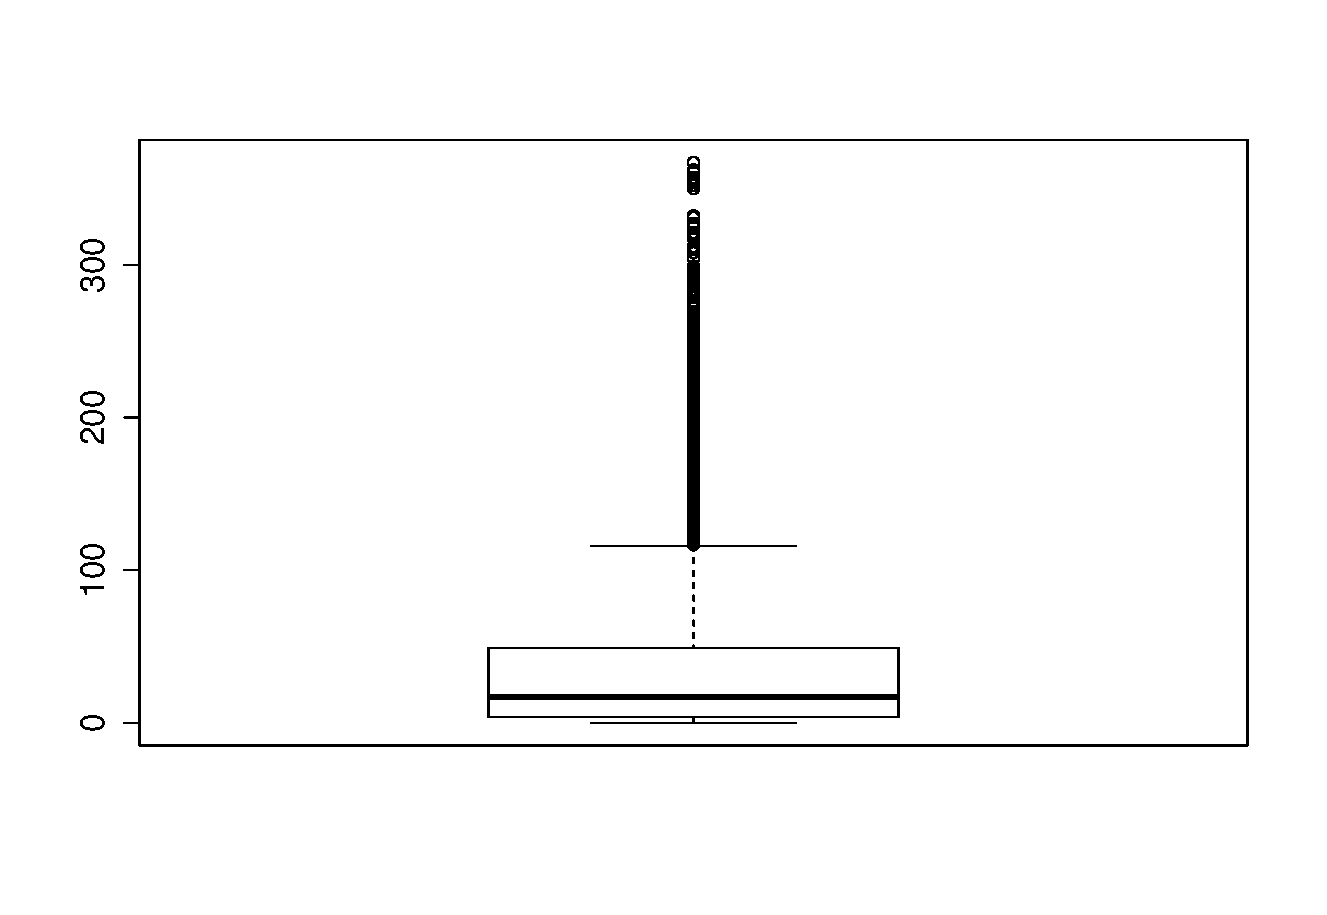
\includegraphics[width=.5\columnwidth]{images/class/boxplot-casual.eps}
  \caption{Boxplot per \texttt{train\$casual}}
  \label{fig:simplest-linear-model}
\end{figure}

Come si può vedere in figura, i dati sono molto concentrati verso valori bassi
di utilizzo (con mediana 18, trovata con il comando \texttt{summary} di R).
Guardando il boxplot, si sceglie 50 come soglia per distinguere se l'utilizzo
è elevato o meno\footnote{N.B. la soglia è puramente arbitraria}.

A questo punto si procede inserendo nel nostro workspace una variabile
``\texttt{aLotCasual}'' che avrà valori 1 o 0 a seconda che il servizio sia
stato utilizzato abbondantemente o meno da utenti non registrati (script
\ref{sec:script-populate-class}).

%%%%%%%%%%%%%%%%%%%%%%%%%%%%%%%%%%%%%%%%%%%%%%%%%%%%%%%%%%%%%%%%%%%%%%%%%%%%%%%
%%%%%%%%%%%%%%%%%%%%%%%%%%%%%%%%%%%%%%%%%%%%%%%%%%%%%%%%%%%%%%%%%%%%%%%%%%%%%%%

\subsection{Regressione lineare logistica}\label{sec:class-log-reg}

Come al solito, si parte sempre tentando di approssimare i nostri dati nel
modo più semplice possibile, ovvero con una retta.

In questo caso però è più conveniente utilizzare, anzichè la regressione
lineare semplice, quella logistica: in questo modo tutti i valori che verranno
predetti dal nostro modelli saranno compresi tra 0 e 1.

Si procede con questo metodo grazie allo script \texttt{logistic-regression.R}
(sez. \ref{sec:script-log-reg}), il quale mostra anche la tabella di errata
classificazione, le curve Lift e ROC.

\begin{table}[H]
\begin{center}
\begin{tabular}{ | l || c | c | }
  \hline
    Previsti/Osservati & 0 & 1 \\ \hline \hline
    0 & 3883 & 293 \\ \hline
    1 & 253 & 1014 \\ \hline
\end{tabular}
  \caption{Tabella di errata classificazione per regressione logistica}
\end{center}
\end{table}

\begin{figure}[H]
  \begin{subfigure}{0.4\textwidth}
    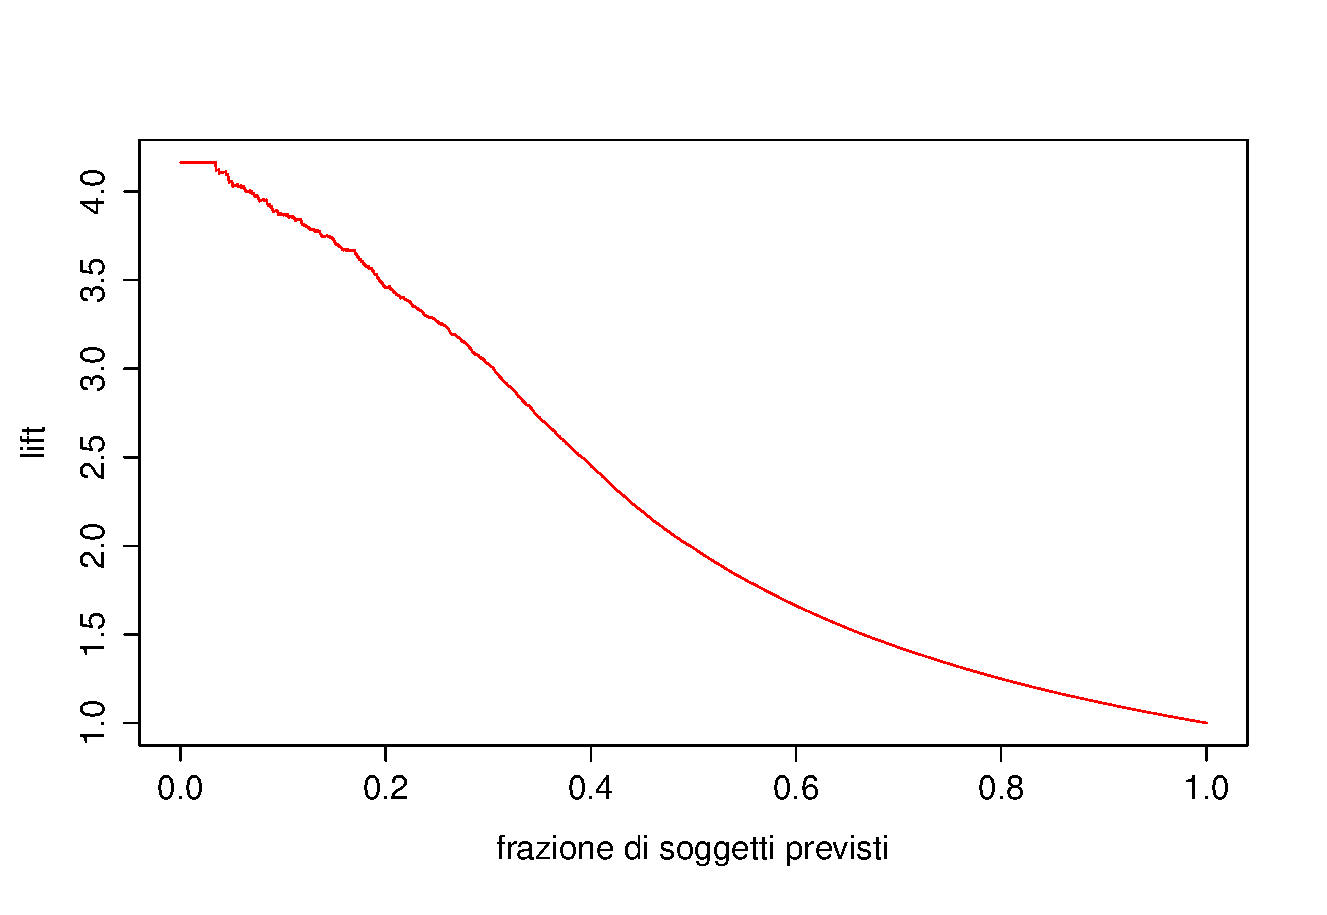
\includegraphics[width=\columnwidth]{images/class/lift-log-reg.eps}
  \end{subfigure}
  \hspace*{\fill}
  \begin{subfigure}{0.4\textwidth}
    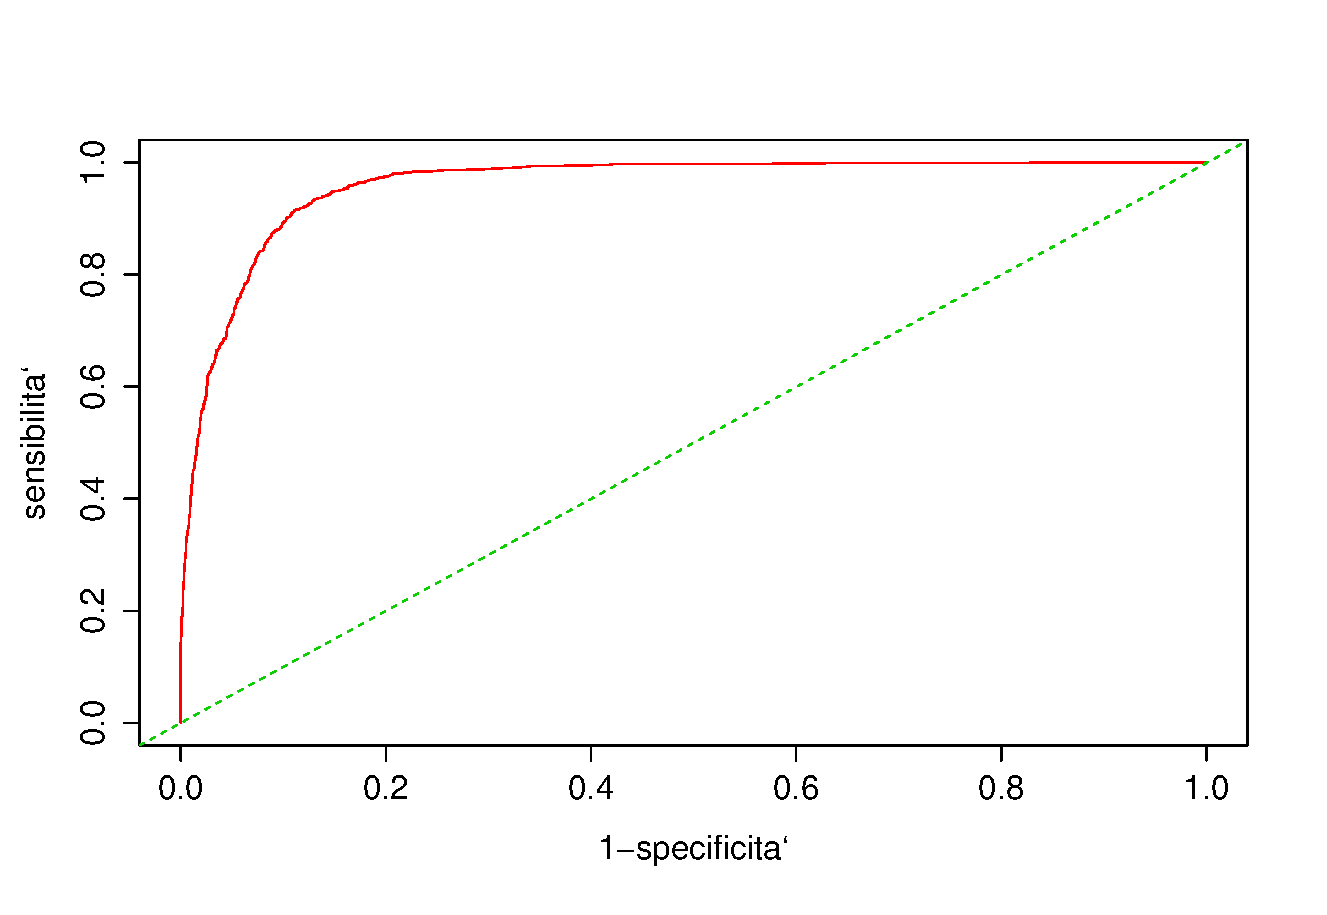
\includegraphics[width=\columnwidth]{images/class/roc-log-reg.eps}
  \end{subfigure}
  \caption{Curve per classificazione con regressione logistica}
  \label{fig:class-reg-1og}
\end{figure}

Analizzando il modello ottenuto, è possibile vedere che i fattori che più
influenzano il nostro nuovo caso di studio sono:

\begin{itemize}
\item \texttt{workingday}: come è normale aspettarsi, è la più significativa.\\
  Il numero di volte che il servizio è stato utilizzato in giorni lavorativi
  da utenti non registrati cala, poichè ci si aspetta che la maggior parte
  degli utenti casuali non risieda in Brooklyn;
\item \texttt{humidity}, al cui crescere il servizio è meno utilizzato spesso
  da utenti non registrati. \\
  Tale risultato può sembrare sensato, poichè anche nelle precedenti sezioni
  abbiamo visto che all'aumentare della temperatura il servizio veniva
  utilizzato di meno in generale nell'afosa Brooklyn;
\item \texttt{temp}: al crescere della temperatura, il servizio viene in
  generale utilizzato maggiormente e tale trend viene confermato;
\item \texttt{atemp}: come per \texttt{temp};
\item \texttt{weather}: al peggiorare delle condizioni metereologiche, il
  servizio viene utilizzato di meno da utenti non registrati. \\
  Anche questo pare sensato, poichè con condizioni metereologiche ci si
  aspetta che sia l'afflusso di turisti (i principali presupposti utenti non
  registrati) a diminuire.
\end{itemize}

%%%%%%%%%%%%%%%%%%%%%%%%%%%%%%%%%%%%%%%%%%%%%%%%%%%%%%%%%%%%%%%%%%%%%%%%%%%%%%%
%%%%%%%%%%%%%%%%%%%%%%%%%%%%%%%%%%%%%%%%%%%%%%%%%%%%%%%%%%%%%%%%%%%%%%%%%%%%%%%

\subsection{MARS}\label{sec:class-mars}

Come secondo tentativo, decidiamo di utilizzare un modello che avevamo già
utilizzato per predire la richiesta del servizio di \emph{Bike sharing} nelle
sezioni precedenti, ovvero MARS.

In questo caso cambia poco da quanto già detto in sezione \ref{sec:mars}, lo
script utilizzato è \texttt{mars-classif.R} (sezione
\ref{sec:script-mars-classif}) e anche questo usa gli stessi strumenti visti
nella sezione \ref{sec:class-log-reg} per valutare la classificazione ottenuta.

\begin{table}[H]
\begin{center}
\begin{tabular}{ | l || c | c | }
  \hline
    Previsti/Osservati & 0 & 1 \\ \hline \hline
    0 & 3907 & 384 \\ \hline
    1 & 211 & 941 \\ \hline
\end{tabular}
  \caption{Tabella di errata classificazione per MARS}
\end{center}
\end{table}

\begin{figure}[H]
  \begin{subfigure}{0.4\textwidth}
    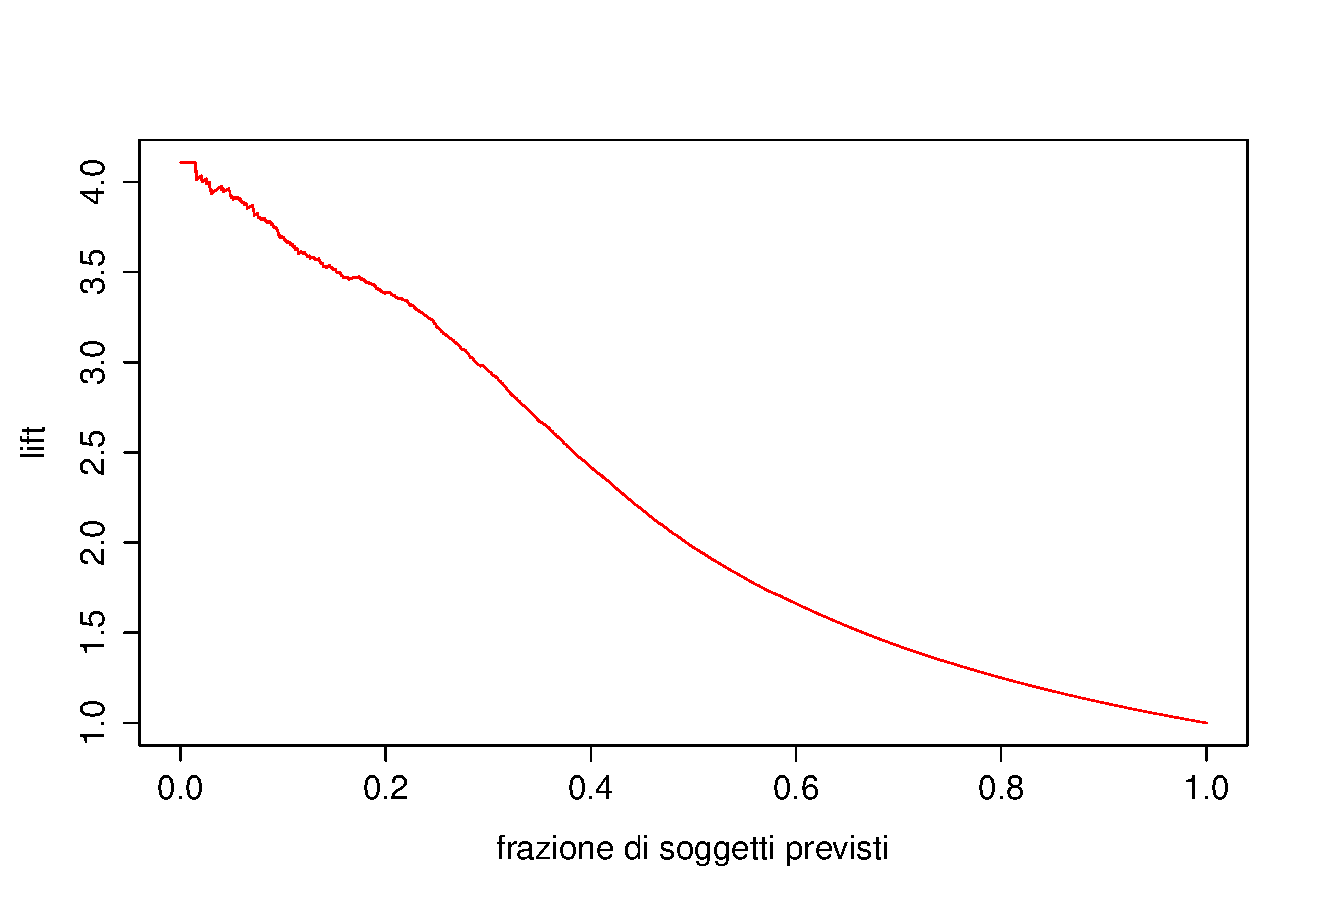
\includegraphics[width=\columnwidth]{images/class/lift-mars.eps}
  \end{subfigure}
  \hspace*{\fill}
  \begin{subfigure}{0.4\textwidth}
    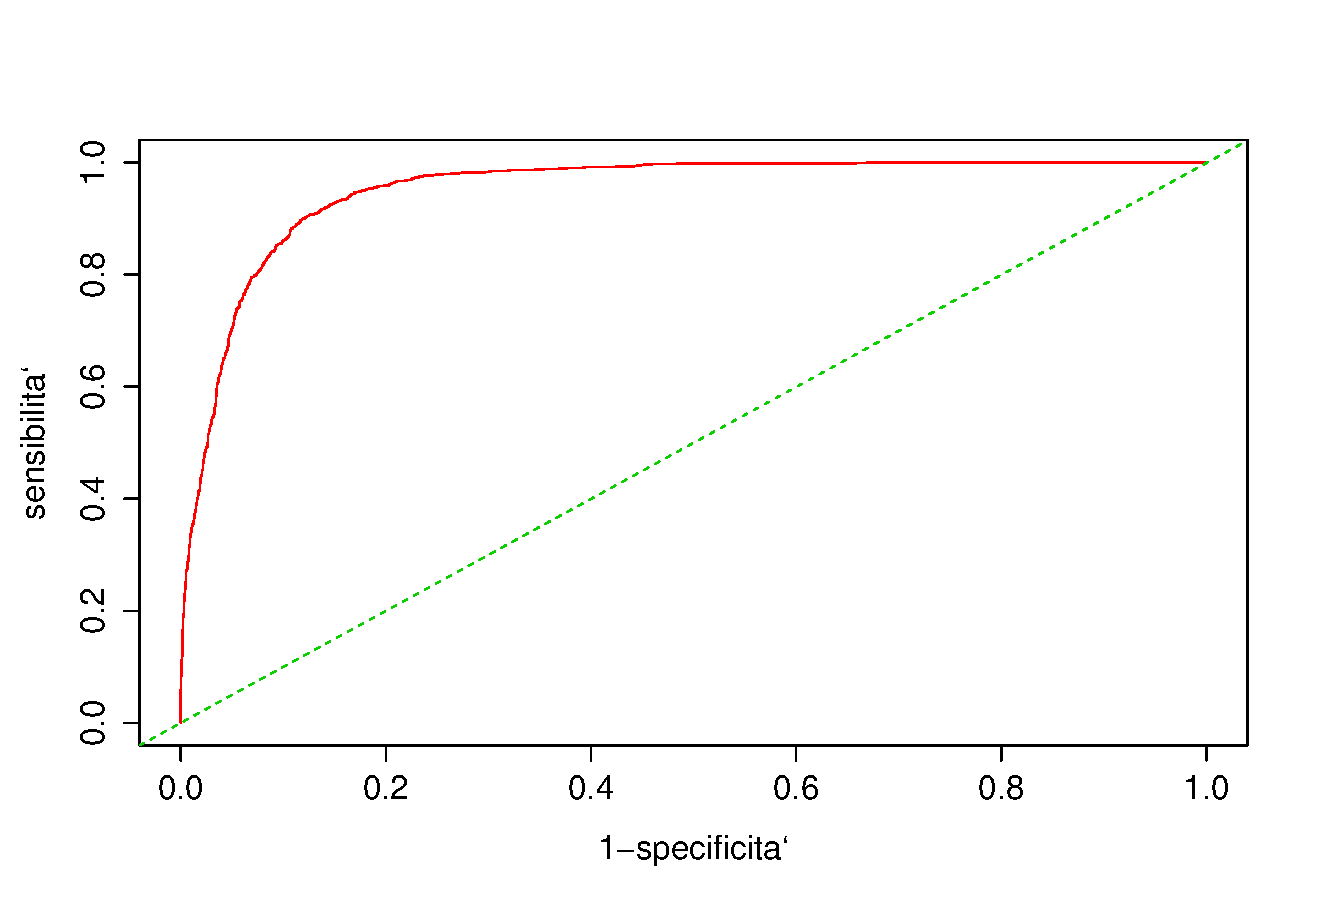
\includegraphics[width=\columnwidth]{images/class/roc-mars.eps}
  \end{subfigure}
  \caption{Curve per classificazione con MARS}
  \label{fig:class-reg-1og}
\end{figure}

Richiedendo il grafico delle variabili più importanti per questo modello
(trovate con il comando \texttt{evimp}), \texttt{temp} e \texttt{workingday}
si confermano le più importanti per questo particolare caso di studio.

%%%%%%%%%%%%%%%%%%%%%%%%%%%%%%%%%%%%%%%%%%%%%%%%%%%%%%%%%%%%%%%%%%%%%%%%%%%%%%%
%%%%%%%%%%%%%%%%%%%%%%%%%%%%%%%%%%%%%%%%%%%%%%%%%%%%%%%%%%%%%%%%%%%%%%%%%%%%%%%

\subsection{GAM}\label{sec:class-gam}

Come terzo tentativo, anche in questo caso decidiamo di utilizzare un modello
che avevamo già utilizzato per predire la richiesta del servizio di \emph{Bike sharing} nelle sezioni precedenti, ovvero GAM.

Pure in questo caso cambia poco da quanto già detto in sezione \ref{sec:gam},
lo script utilizzato è \texttt{gam-classif.R} (sezione
\ref{sec:script-gam-classif}) e anche questo usa gli stessi strumenti visti
nella sezione \ref{sec:class-log-reg} per valutare la classificazione ottenuta.

\begin{table}[H]
\begin{center}
\begin{tabular}{ | l || c | c | }
  \hline
    Previsti/Osservati & 0 & 1 \\ \hline \hline
    0 & 3866 & 277 \\ \hline
    1 & 252 & 1048 \\ \hline
\end{tabular}
  \caption{Tabella di errata classificazione per GAM}
\end{center}
\end{table}

\begin{figure}[H]
  \begin{subfigure}{0.4\textwidth}
    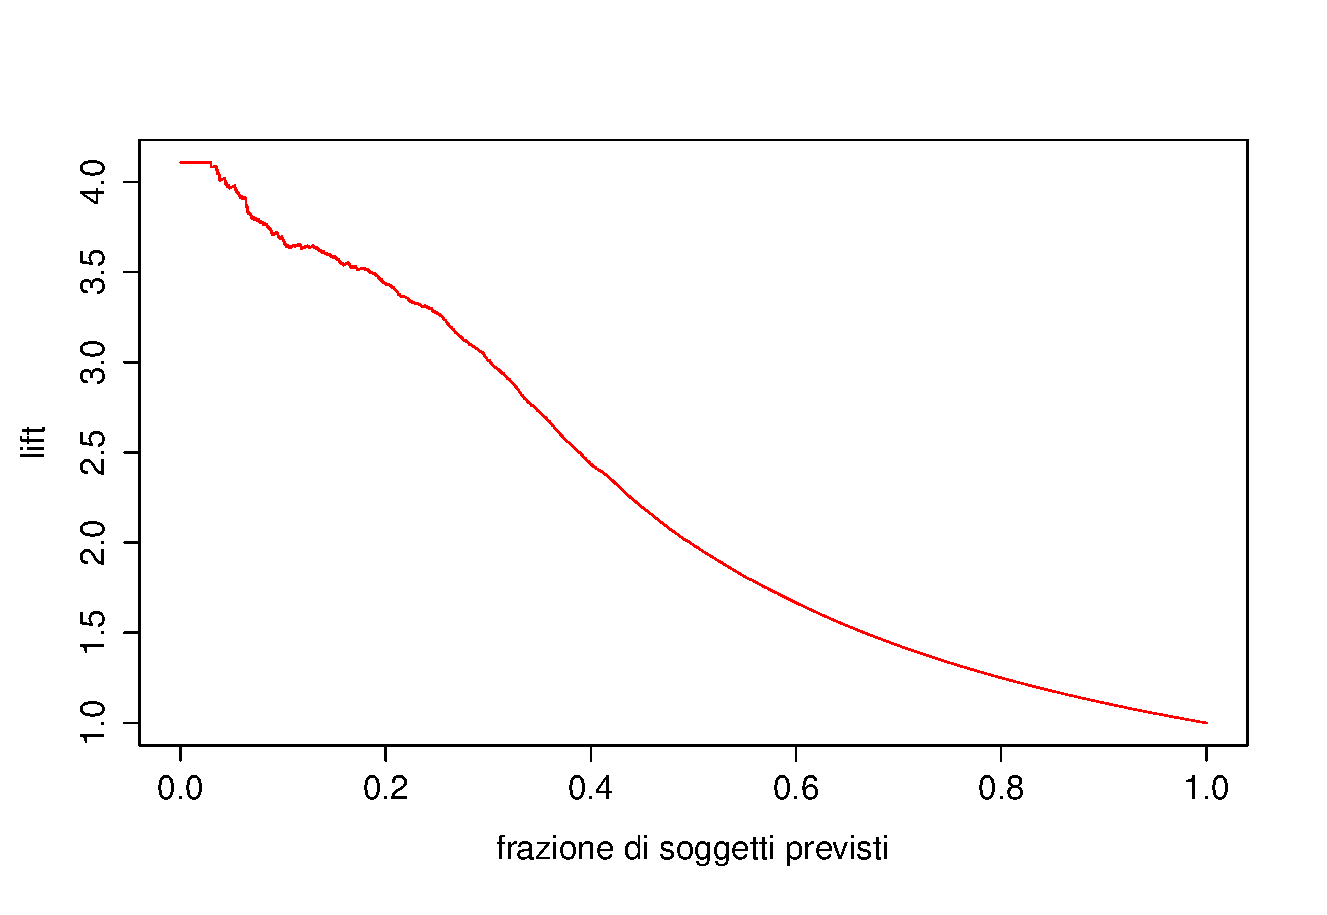
\includegraphics[width=\columnwidth]{images/class/lift-gam.eps}
  \end{subfigure}
  \hspace*{\fill}
  \begin{subfigure}{0.4\textwidth}
    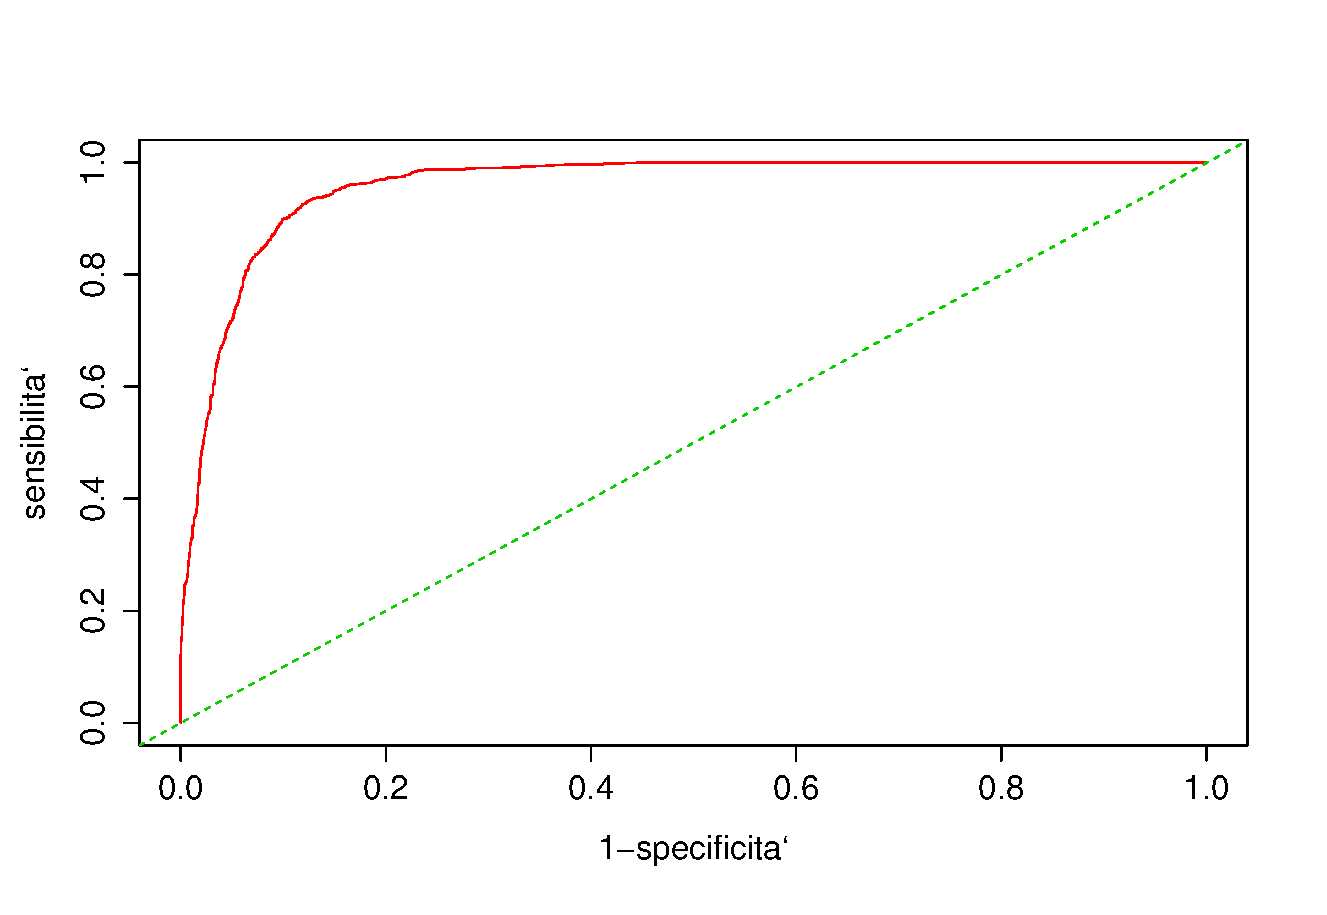
\includegraphics[width=\columnwidth]{images/class/roc-gam.eps}
  \end{subfigure}
  \caption{Curve per classificazione con GAM}
  \label{fig:class-reg-1og}
\end{figure}

Come nella sezione \ref{sec:class-mars}, le variabili più significative sono
\texttt{temp} e \texttt{workingday}.

Tuttavia, dal grafico di questo modello se un giorno è lavorativo, la
richiesta del servizio da parte di utenti non registrati cala, mentre
all'aumentare della temperatura la richiesta cresce. \\
Si ritiene che ciò sia dovuto al fatto che il più delle volte la temperatura è
sufficiente da sola per determinare una richiesta alta di \emph{Bike sharing}
da parte di qualsiasi tipo di utente e che in questo caso le altre variabili
agiscano per ``bilanciare'' l'effetto della temperatura.

%%%%%%%%%%%%%%%%%%%%%%%%%%%%%%%%%%%%%%%%%%%%%%%%%%%%%%%%%%%%%%%%%%%%%%%%%%%%%%%
%%%%%%%%%%%%%%%%%%%%%%%%%%%%%%%%%%%%%%%%%%%%%%%%%%%%%%%%%%%%%%%%%%%%%%%%%%%%%%%

\subsection{Reti neurali}\label{sec:class-nnet}

Come quarto tentativo, anche in questo caso decidiamo di utilizzare un modello
che avevamo già utilizzato per predire la richiesta del servizio di \emph{Bike
sharing} nelle sezioni precedenti, ovvero una rete neurale.

Pure in questo caso cambia poco da quanto già detto in sezione
\ref{sec:neural-nets}, lo script utilizzato è \texttt{nnet-classif.R} (sezione
\ref{sec:script-nnet-classif}) e anche questo usa gli stessi strumenti visti
nella sezione \ref{sec:class-log-reg} per valutare la classificazione ottenuta.

\begin{table}[H]
\begin{center}
\begin{tabular}{ | l || c | c | }
  \hline
    Previsti/Osservati & 0 & 1 \\ \hline \hline
    0 & 3884 & 186 \\ \hline
    1 & 275 & 1098 \\ \hline
\end{tabular}
  \caption{Tabella di errata classificazione per rete neurale}
\end{center}
\end{table}

\begin{figure}[H]
  \begin{subfigure}{0.4\textwidth}
    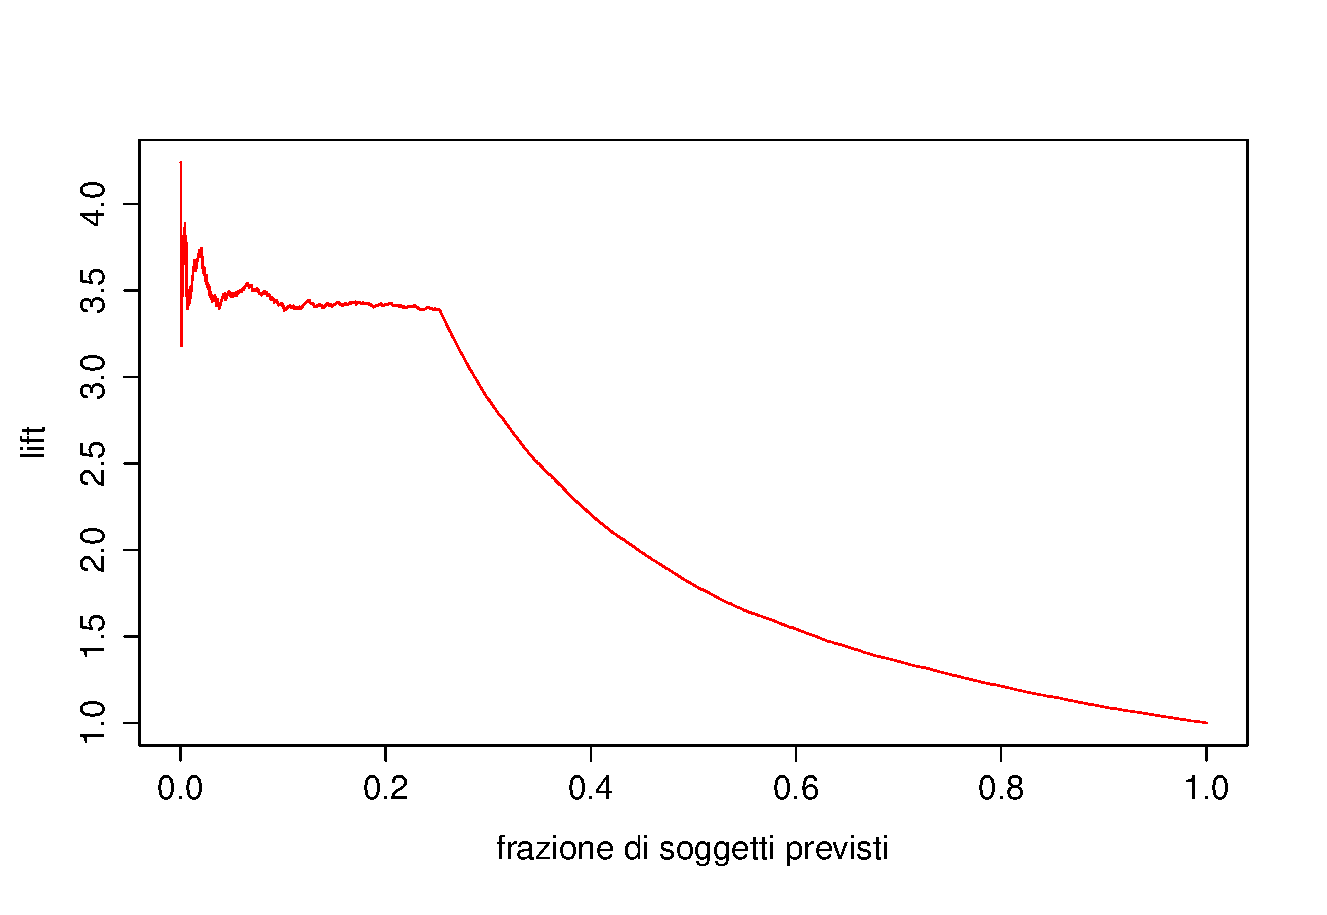
\includegraphics[width=\columnwidth]{images/class/lift-nnet.eps}
  \end{subfigure}
  \hspace*{\fill}
  \begin{subfigure}{0.4\textwidth}
    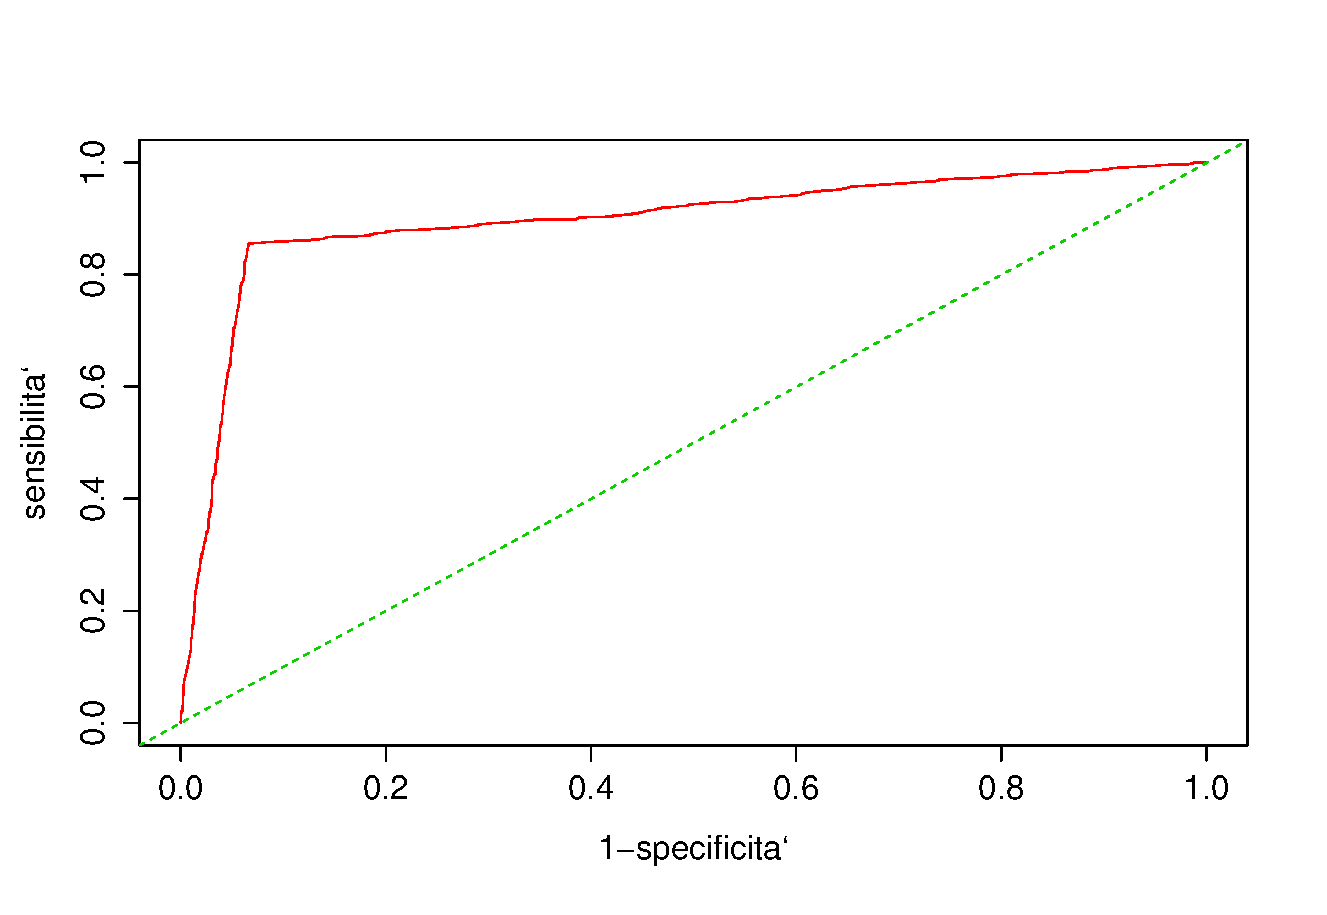
\includegraphics[width=\columnwidth]{images/class/roc-nnet.eps}
  \end{subfigure}
  \caption{Curve per classificazione con rete neurale}
  \label{fig:class-reg-1og}
\end{figure}

Come è possibile vedere dalla figura \ref{fig:nnet} (per questo modello non
viene riportata la rete neurale finale), le reti neurali non sono facili da
interpretare, quindi per valutarne l'efficacia utilizzeremo in seguito
solamente le curve Lift e ROC.

%%%%%%%%%%%%%%%%%%%%%%%%%%%%%%%%%%%%%%%%%%%%%%%%%%%%%%%%%%%%%%%%%%%%%%%%%%%%%%%
%%%%%%%%%%%%%%%%%%%%%%%%%%%%%%%%%%%%%%%%%%%%%%%%%%%%%%%%%%%%%%%%%%%%%%%%%%%%%%%

\subsection{Reti neurali}\label{sec:class-nnet}

L'ultimo modello utilizzato è un albero di regressione.

Pure in questo caso cambia poco da quanto già detto in sezione
\ref{sec:trees}, lo script utilizzato è \texttt{tree-classif.R} (sezione
\ref{sec:script-tree-classif}) e anche questo usa gli stessi strumenti visti
nella sezione \ref{sec:class-log-reg} per valutare la classificazione ottenuta.

\begin{table}[H]
\begin{center}
\begin{tabular}{ | l || c | c | }
  \hline
    Previsti/Osservati & 0 & 1 \\ \hline \hline
    0 & 3755 & 238 \\ \hline
    1 & 345 & 1105 \\ \hline
\end{tabular}
  \caption{Tabella di errata classificazione per albero di regressione}
\end{center}
\end{table}

\begin{figure}[H]
  \begin{subfigure}{0.4\textwidth}
    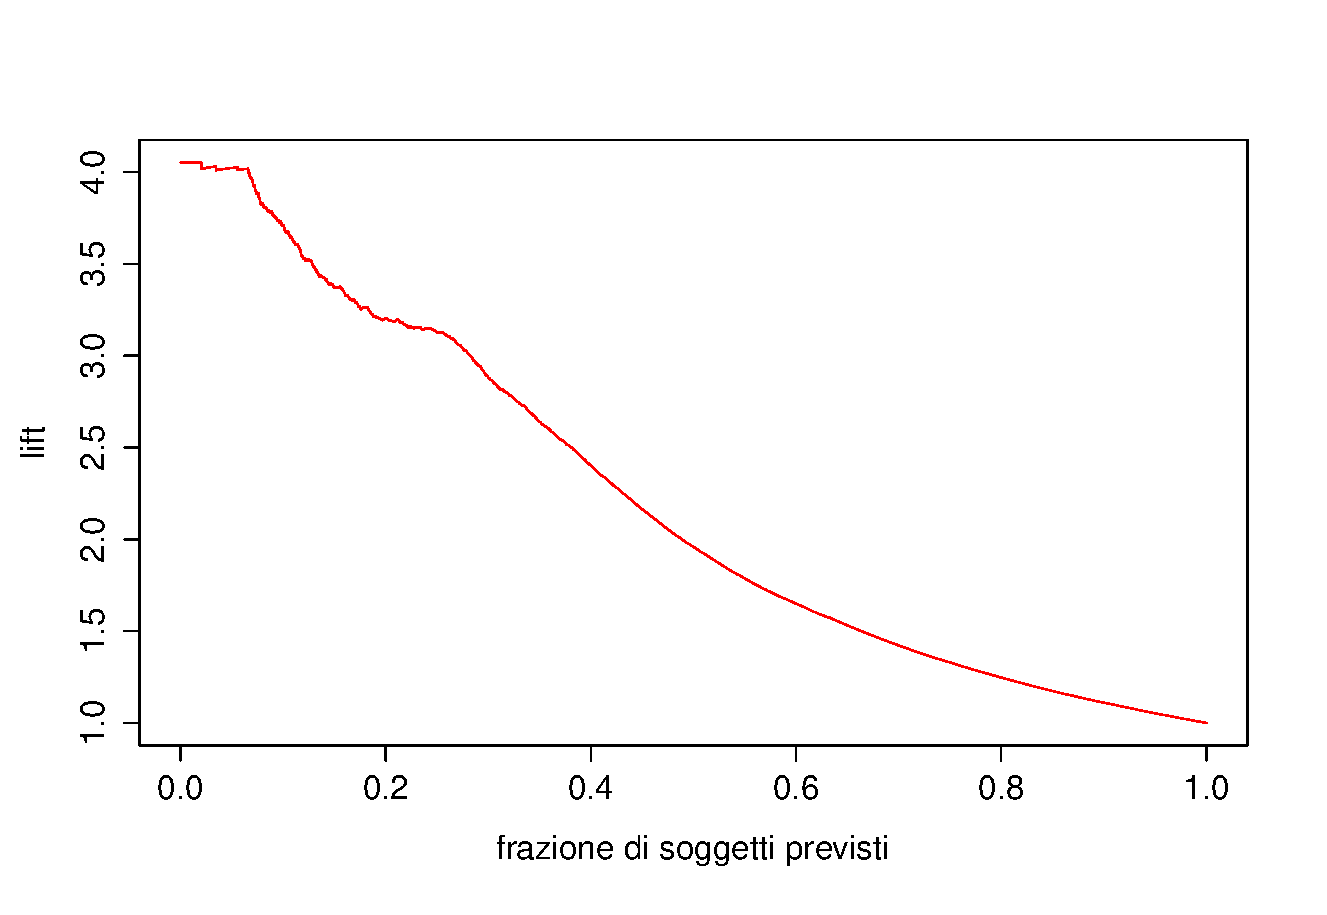
\includegraphics[width=\columnwidth]{images/class/lift-tree.eps}
  \end{subfigure}
  \hspace*{\fill}
  \begin{subfigure}{0.4\textwidth}
    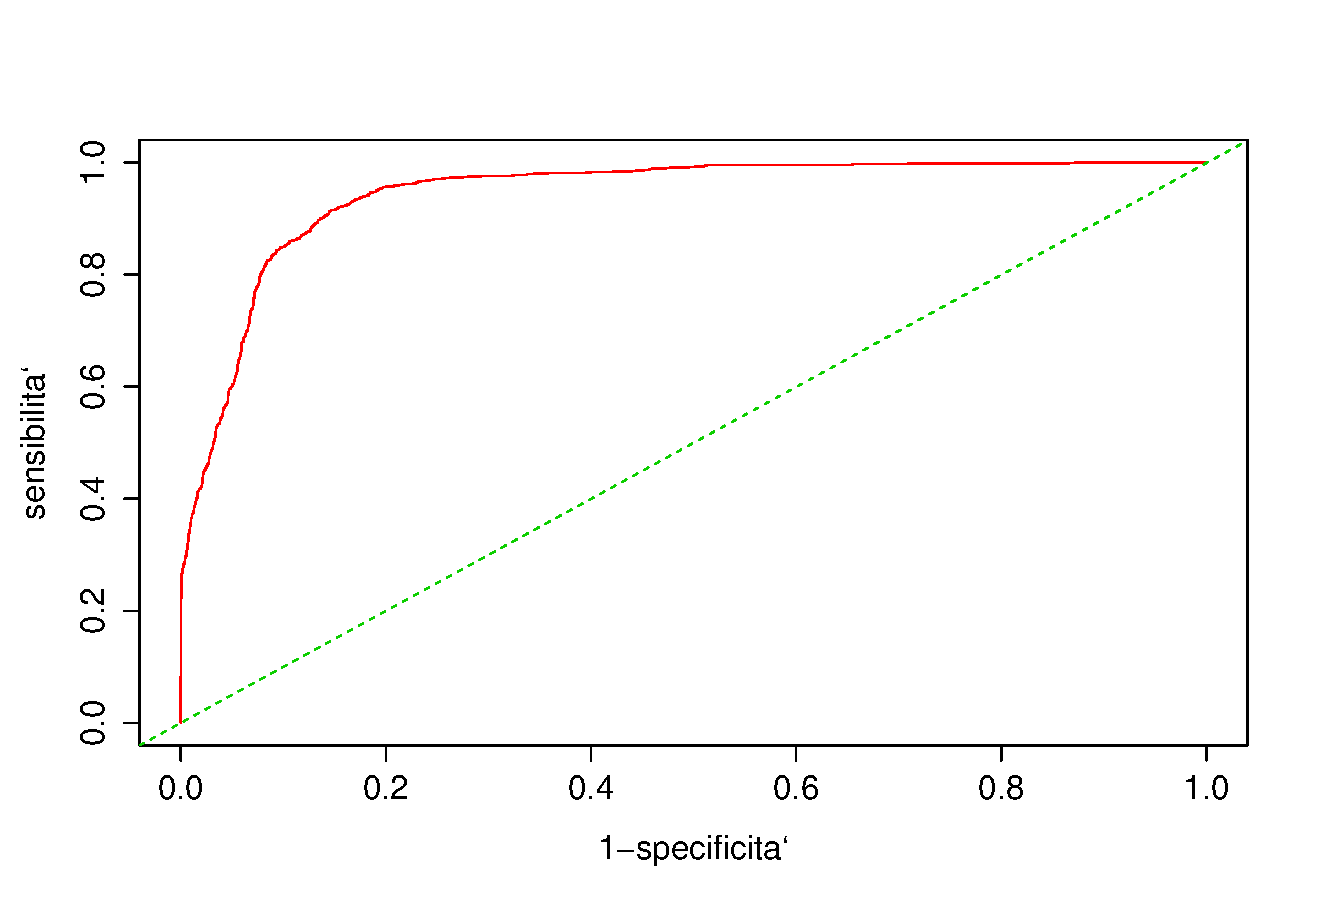
\includegraphics[width=\columnwidth]{images/class/roc-tree.eps}
  \end{subfigure}
  \caption{Curve per classificazione con albero di regressione}
  \label{fig:class-reg-1og}
\end{figure}

Come è possibile vedere dalla figura \ref{fig:nnet} (per questo modello non
viene riportata la rete neurale finale), le reti neurali non sono facili da
interpretare, quindi per valutarne l'efficacia utilizzeremo in seguito
solamente le curve Lift e ROC.
